\documentclass{article}
\usepackage{graphicx}
\usepackage{polski}
\usepackage[utf8]{inputenc}
\usepackage{graphicx}

\usepackage{subcaption}
\usepackage{algpseudocode}


\usepackage[a5paper]{geometry}
\graphicspath{ {./wykresy/} }
\begin{document}
\title{Model Chandrasekhara / Smoluchowskiego  - 1 pudełko}
\author{Piotr Piękos}

\maketitle

\section{Oznaczenia}
W celach notacyjnych rozbijemy proces $X(t)$ (ilość żyjących osób) na dwa procesy: 
\begin{itemize}
\item$N(t)$ - Ilość narodzin
\item$S(t)$ - Ilość śmierci
\end{itemize}
Wtedy $X(t) = N(t) - S(t)$,
Dodatkowo oznaczymy intensywności procesów przez:
\begin{itemize}
\item$a_N$ - intensywność procesu narodzin
\item$a_S$ - parametr rozkładu wykładniczego odpowiadającego za długość życia
\end{itemize}
Dodatkowe oznaczenia:
\begin{itemize}
\item$I_X(t)$ - indeksy "żywych" zmiennych w momencie t.
\item$W_i$ - zmienna losowa (o rozkładzie wykladniczym z parametrem $a_S$) mówiąca o długości życia osoby $i$
\end{itemize}

Możnaby spróbować zamodelować $S(t)$ jako niejednorodny proces Poissona z intensywnością zależną od $N(t)$. Ja jednak to rozdzieliłem jedynie ze względów notacyjnych.

\section{Prawa ewolucji}
$P(X(t+h) = x + 1 | X(t) = 1)$:

Korzystamy tutaj z faktu, że dla procesu Poissona (N) mamy: 
\begin{itemize}
\item $P(N(t+h) = n + 1 | N(t) = n) = a_N h + o(h)$
\item $P(N(t+h) \geq n + 2 | N(t) = n) = o(h)$
\end{itemize}
Dodatkowo:
\begin{itemize}
\item $P(N(t+h) = n | N(t) = n) = 1 - a_N h + o(h)$
\item $P(S(t+h) = s | S(t) = s, X(t) = x) = P(\forall_i \in I_X(t) W_i \geq h) + o(h) = \prod_{i \in I_X(t)} P(W_i \geq h) + o(h) = e^{-a_Sxh} + o(h) = 1 - a_Sxh + o(h)$
\item $P(S(t+h) = s+1 | S(t) = s, X(t) = x) = x(e^{-a_S(x-1)h} - e^{-a_Sxh}) + o(h) = a_Sxh + o(h)$
\item $P(S(t+h) = s+2 | S(t) = s, X(t) = x) = o(h)$
\end{itemize}
$o(h)$ pojawia się już po pierwszej równości ze względu na to, że przy dokładnym rozpisaniu prawdopodobienstw należałoby warunkować w którym momencie X(t) się zmieni (X jest zależny od S), jednak ta różnica jest $o(h)$, więc po prostu jest zawarta w tym.

zatem
\[P(X(t+h) = x+1 | X(t) = x) = \]
\[P(N(t+h) = n + 1 | N(t) = n) \cdot P(S(t+h) = s| S(t) = s, X(t)=x) = \]
\[(a_N h + o(h)) \cdot (1 - a_Sxh + o(h)) = \]
\[a_N h + o(h) \] 

\[P(X(t+h) = x-1 | X(t) = x) = \]
\[P(N(t+h) = n | N(t) = n) \cdot P(S(t+h) = s+1| S(t) = s, X(t)=x) = \]
\[(1 - a_N h + o(h)) \cdot (a_Sxh + o(h)) = \]
\[a_S xh + o(h) \] 

Czyli mamy \begin{itemize}
\item$P(X(t+h) = x+1 | X(t) = x) = a_N h + o(h)$
\item$P(X(t+h) = x-1 | X(t) = x) = a_S xh + o(h)$
\end{itemize}
wzory te razem z $Q(x,x) = -a_Nh - a_Sxh$ i zerami w pozostałych wierszach opisują intensywność przejść procesu Markowa
\section{Symulacje}
\subsection{Algorytm}
Algorytm symulacji składa się z dwóch części: \begin{enumerate}
\item standardowa symulacja procesu Poissona (czasy narodzin)
\item symulacja czasów życia z rozkładu wykładniczego o parametrze $a_S$
\end{enumerate}
Konkretnie:


\begin{algorithmic}
\State Gen $N \sim \textit{Poiss}(a_Nt)$
\State for $i = 1$ to N do Gen $U_i \sim U(0, t)$, Gen $L_i \sim \textit{Exp}(1/a_S)$
\State $(T_1, ..., T_n) =$ Sort$(U_1, ..., U_n)$ otrzymujemy proces Poissona, czasy narodzin
\State $(D_1, ..., D_n) = (T_1 + L_1, ..., T_n + L_n)$ - dodajemy niezalezne czasy zycia do czasow narodzin i mamy czasy smierci.
\end{algorithmic}  


Algorytm korzysta z gotowych bibliotek (numpy) do symulacji rozkładów Poissona i rozkładu wykładniczego. Dodatkowo wykorzystuje w nich możliwość wektoryzacji. Ale można to zrobić surowo od rozkładu jednostajnego np. za pomocą metody odwracania dystrybuanty oraz chociażby metody eliminacji.

\subsection{Przykładowe trajektorie}

\begin{figure}[h!]
\centering
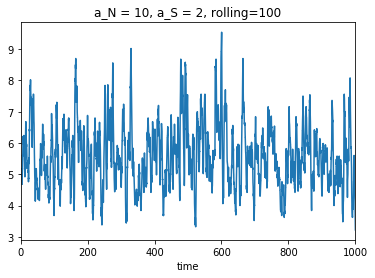
\includegraphics[width=0.4\linewidth]{10,2}
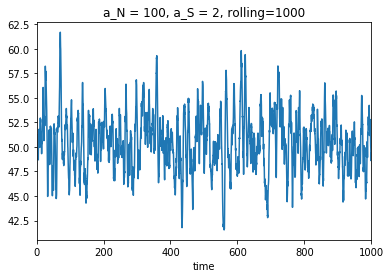
\includegraphics[width=0.4\linewidth]{100,2}
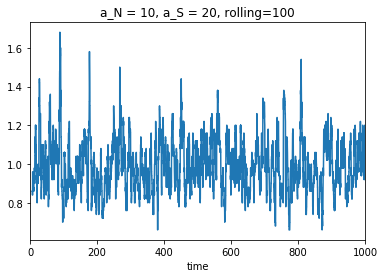
\includegraphics[width=0.4\linewidth]{10,20}
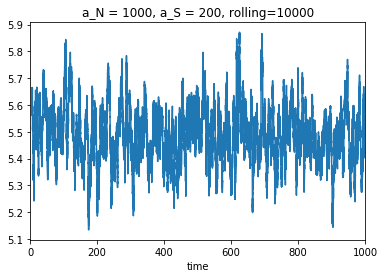
\includegraphics[width=0.4\linewidth]{1000,200}
\caption{Przykładowe trajektorie symulacji}
\end{figure}
Wygenerowane wykresy są sparametryzowane 3 parametrami: \begin{itemize}
\item $a\_N - a_N$
\item $a\_S - a_S$
\item rolling - długość horyzontu średniej kroczącej, średnia krocząca jest konieczna dla wielu wykresów ze względu na ogromną ilośc punktów na wykresie. Pokazuje jednak ona "gęstość" punktów.
\end{itemize}
W trajektoriach należy także zwrócić uwagę na skalę, gdyż ona odgrywa kluczową rolę.

Od razu widać, że wyróżnioną liczbą jest $\frac{a_N}{a_S}$. Proces oscyluje w jej okolicach, co jest zrozumiałe po spojrzeniu na prawa ewolucji. Mówią one, że punkt $\frac{a_N}{a_S}$ jest punktem granicznym dla którego intensywność śmierci jest taka sama jak intensywność narodzin. 

Możnaby pokusić się o alternatywną parametryzację procesu za pomocą parametrów $a = \frac{a_N}{a_S}$ i $b = a_S$, wtedy $a$ reprezentowałaby punkt w okół którego symulacja będzie oscylować, a b reprezentowałby gęstość punktow.

Skyupmy się teraz na dwóch procesach o tym samym parametrze $a (\frac{a_N}{a_S}$. Są widoczne na pierwszym i ostatnim wykresie wyżej ($\frac{a_N}{a_S} = 5)$. Na wykresach widać po pierwsze większy parametr rolling który jest konieczny ze względu na większa gęstość punktów. Z tych wykresów możnaby też odczytać, że gęstszy wykres ma mniejsze odchylenia, jednak byłoby to błędne, gdyż jest to spowodowane jedynie wygładzeniem przez średnią kroczącą.
\section{Analiza}
\subsection{Istnienie rozkładu stacjonarnego}
\subsection{Wartość oczekiwana}
\subsection{Wyliczenie rozkładu stacjonarnego}
\end{document}